\documentclass[ dottedtoc,oneside,openright,titlepage,numbers=noenddot,headinclude,letterpaper
                footinclude=true,cleardoublepage=empty,abstractoff,
                paper=letterpaper,fontsize=12pt,
                ngerman,american,
                ]{scrreprt}

%********************************************************************
% Note: Make all your adjustments in here
%*******************************************************
\usepackage{algorithm}% http://ctan.org/pkg/algorithms
\usepackage{algpseudocode}% http://ctan.org/pkg/algorithmicx

\usepackage{comment}
\usepackage{adjustbox}
\usepackage[section]{placeins}
\usepackage{listings}
\usepackage{longtable}
\usepackage{colortbl}
\usepackage{caption}
\usepackage{setspace}
% *****************************************************************************
% Triggers for this config
% *****************************************************************************
\usepackage{ifthen}
\newboolean{enable-backrefs} % enable backrefs in the bibliography
\setboolean{enable-backrefs}{false} % true false
% *****************************************************************************


% *****************************************************************************
% 2. Personal data and user ad-hoc commands
% *****************************************************************************
\newcommand{\invpyr}[1]{\vbox{\hsize=4.5in \parindent=0pt \emergencystretch=1in
  \parshape 6
    0.00in 4.50in
    0.25in 4.00in
    0.50in 3.50in
    0.75in 3.00in
    1.00in 2.50in
    1.25in 2.00in
    \leftskip=0pt plus 1fil \rightskip=0pt plus -1fil
    \parfillskip=0pt plus 2fil
    #1}}


\newcommand{\myTitle}{Your Thesis title here \xspace}
\newcommand{\myTITLE}{\expandafter\MakeUppercase\expandafter{\myTitle}}


\newcommand{\mySubtitle}{\singlespacing A thesis submitted to the Graduate
College of \\ 
Texas State University in partial fulfillment \\
of the requirements for the degree of\\}
\newcommand{\myDegree}{Master of Science \\ with a Major in Computer Science\xspace}


\newcommand{\myName}{Your Name Here\xspace}
\newcommand{\myProf}{Put professor here\xspace}
\newcommand{\myOtherProf}{Put name here\xspace}
\newcommand{\mySupervisor}{You Advisor\xspace}
\newcommand{\myFaculty}{Put data here\xspace}
\newcommand{\myDepartment}{Department of Computer Science\xspace}
\newcommand{\myUni}{Texas State University\xspace}
\newcommand{\myLocation}{San Marcos\xspace}
\newcommand{\myTime}{December 2020\xspace}  %\myTime Must be either May or December
\newcommand{\myYear}{2020\xspace}
\newcommand{\myVersion}{version 4.1\xspace}
\newcommand{\myCommitteeOne}{Committee Member 1, Chair\xspace}
\newcommand{\myCommitteeTwo}{Committee Member 2\xspace}
\newcommand{\myCommitteeThree}{Committee Member 3 \xspace}


% *****************************************************************************
% Setup, finetuning, and useful commands
% *****************************************************************************
\newcounter{dummy} % necessary for correct hyperlinks (to index, bib, etc.)
\newlength{\abcd} % for ab..z string length calculation
\newcommand{\ie}{i.\,e.}
\newcommand{\Ie}{I.\,e.}
\newcommand{\eg}{e.\,g.}
\newcommand{\Eg}{E.\,g.} 
% *****************************************************************************


% *****************************************************************************
% 3. Loading some handy packages
% *****************************************************************************
\PassOptionsToPackage{latin9}{inputenc}
 \usepackage{inputenc}
\PassOptionsToPackage{square}{natbib}
 \usepackage[numbers]{natbib}
\PassOptionsToPackage{fleqn}{amsmath}   % math environments and more by the AMS
 \usepackage{amsmath}
\DeclareMathOperator*{\argmax}{argmax}
\PassOptionsToPackage{T1}{fontenc}
    \usepackage{fontenc}

% *****************************************************************************
% General useful packages
% *****************************************************************************
\usepackage{textcomp} % fix warning with missing font shapes
\usepackage{scrhack} % fix warnings when using KOMA with listings package
\usepackage{xspace} % to get the spacing after macros right
\usepackage{fixltx2e} % fixes some LaTeX stuff 
\PassOptionsToPackage{printonlyused,smaller}{acronym}
	\usepackage{acronym} % nice macros for handling all acronyms in the thesis



%\usepackage{scrpage2}
\usepackage{tocloft}


%******************************************************************************
% The following are all hacks for the Table of Contents
%******************************************************************************
% spacing before contents heading
\setlength{\cftbeforetoctitleskip}{-2em}
% dotted leaders for chapters
\renewcommand{\cftchapleader}{\cftdotfill{\cftdotsep}}
\renewcommand{\cftpartleader}{\cftdotfill{\cftdotsep}}

% center, regular font, bold title, for Table of Contents
\renewcommand{\cfttoctitlefont}{}
\renewcommand{\contentsname}{\hfill\bfseries TABLE OF CONTENTS\hfill}
\renewcommand{\cftaftertoctitle}{\hfill\\\null\hfill\textbf{Page}}
\cftsetindents{tab}{1in}{3in}

% regular font and spacing for parts
\renewcommand{\cftpartfont}{}
\renewcommand{\cftpartpagefont}{}

\setlength{\cftbeforepartskip}{0em}
\setlength{\cftbeforechapskip}{0em}
\setlength{\cftbeforesecskip}{-1em}

% regular font for chapters
\renewcommand{\cftchapfont}{}
\renewcommand{\cftchappagefont}{}

% Add period after chapter number
\renewcommand{\cftchapaftersnum}{.}

% Fixing indentation
\cftsetindents{section}{5.5em}{1.5em}
\cftsetindents{subsection}{6em}{1.5em}
\cftsetindents{chapter}{2em}{2.4em}
\cftsetindents{part}{0in}{.5in}

% Roman numerals for chapters
\renewcommand\thechapter{\Roman{chapter}}

% more hacks to get chapter heading
\newcommand{\mychapter}[2]{
    \setcounter{chapter}{#1}
    \setcounter{section}{0}
    \addcontentsline{toc}{part}{#2}
}

\usepackage{chngcntr}
\counterwithout{figure}{chapter}
\counterwithout{table}{chapter}
\renewcommand{\cftfigaftersnum}{.}
\renewcommand{\cfttabaftersnum}{.}


%******************************************************************************
% List of figures formatting hacks
%******************************************************************************
\setlength{\cftbeforeloftitleskip}{-2em}
% center, regular font, bold title
\renewcommand{\cftloftitlefont}{}
\renewcommand{\listfigurename}{\hfill\bfseries LIST OF FIGURES\hfill}
\renewcommand{\cftafterloftitle}{
\\[1em]\mbox{}\hspace{-13pt}\textbf{Figure} \hfill{\normalfont \textbf{Page}}}

\setlength{\cftaftertoctitleskip}{-1em}
\setlength{\cftafterloftitleskip}{0em}
\setlength{\cftafterlottitleskip}{0em}
\cftsetindents{fig}{0in}{.3in}


%******************************************************************************
% List of tables formatting hacks
%******************************************************************************
\setlength{\cftbeforelottitleskip}{-2em}
% center, regular font, bold title
\renewcommand{\cftlottitlefont}{}
\renewcommand{\cftafterlottitle}{
\\[1em]\mbox{}\hspace{-13pt}\textbf{Table} \hfill{\normalfont \textbf{Page}}}
\cftsetindents{tab}{0in}{.3in}



%******************************************************************************
% Bibliography hacks
%******************************************************************************
\newcommand\mybibname{{\bf REFERENCES}}
\renewcommand\bibsection{%
   \clearpage
   \markboth{\MakeUppercase{\mybibname}}{\MakeUppercase{\mybibname}}%
  }
\def\bibsection{\begin{center}\mybibname\end{center}}
  
%******************************************************************************
% Section and chapter font hacks
%******************************************************************************
\usepackage[explicit]{titlesec}
\usepackage[normalem]{ulem}
\titleformat{\section}{\center\normalfont}{\thesection}{1em}{\uline{#1}}
\titleformat{\chapter}{\center\normalfont\bfseries}{\thechapter .}{1em}{#1}
\titlespacing*{\chapter}{0pt}{-31pt}{40pt}
\titleformat{\subsection}{\normalfont}{\thesubsection}{1em}{\uline{#1}}


% *****************************************************************************
% 4. Setup floats: tables, (sub)figures, and captions
% *****************************************************************************
\usepackage{tabularx} % better tables
	\setlength{\extrarowheight}{3pt} % increase table row height
\usepackage{caption}
\captionsetup{format=hang,font=small}
\usepackage{subfig}
\captionsetup{aboveskip=10pt}
\captionsetup{belowskip=10pt}
% *****************************************************************************


% *****************************************************************************
% 5. Setup code listings
% *****************************************************************************
\usepackage{listings} 
\lstset{language=[LaTeX]Tex,
    keywordstyle=\color{RoyalBlue},
    basicstyle=\small\ttfamily,
    commentstyle=\color{Green}\ttfamily,
    stringstyle=\rmfamily,
    numbers=none,
    numberstyle=\scriptsize,
    stepnumber=5,
    numbersep=8pt,
    showstringspaces=false,
    breaklines=true,
    frameround=ftff,
    frame=single,
    belowcaptionskip=.75\baselineskip
}


% *****************************************************************************
% Using PDFLaTeX
% *****************************************************************************
\PassOptionsToPackage{pdftex,hyperfootnotes=false,pdfpagelabels}{hyperref}
	\usepackage{hyperref}  % backref linktocpage pagebackref
\pdfcompresslevel=9
\pdfadjustspacing=1 
\PassOptionsToPackage{pdftex}{graphicx}
	\usepackage{graphicx} 


% ********************************************************************
% Hyperreferences
% ********************************************************************
\hypersetup{
    draft,	% = no hyperlinking at all (useful in b/w printouts)
    colorlinks=true, linktocpage=true, pdfstartpage=3, pdfstartview=FitV,%
    % uncomment the following line if you want to have black links (e.g., for printing)
    %colorlinks=false, linktocpage=false, pdfborder={0 0 0}, pdfstartpage=3, pdfstartview=FitV,% 
    breaklinks=true, pdfpagemode=UseNone, pageanchor=true, pdfpagemode=UseOutlines,%
    plainpages=false, bookmarksnumbered, bookmarksopen=true, bookmarksopenlevel=1,%
    hypertexnames=true, pdfhighlight=/O,%nesting=true,%frenchlinks,%
    urlcolor=webbrown, linkcolor=RoyalBlue, citecolor=webgreen, %pagecolor=RoyalBlue,%
    %urlcolor=Black, linkcolor=Black, citecolor=Black, %pagecolor=Black,%
    pdftitle={\myTitle},%
    pdfauthor={\textcopyright\ \myName, \myUni, \myFaculty},%
    pdfsubject={},%
    pdfkeywords={},%
    pdfcreator={pdfLaTeX},%
    pdfproducer={LaTeX with hyperref and classicthesis}%
}
% *****************************************************************************
% 7. Last calls before the bar closes
% *****************************************************************************
\listfiles
 
\usepackage[letterpaper,top=2in, bottom=1in, left=1.5in, right=1in]{geometry}
\usepackage[dvipsnames]{xcolor}
%\usepackage{showframe}
\usepackage{indentfirst}


%********************************************************************
% Hyphenation
%*******************************************************

% ********************************************************************
% GO!GO!GO! MOVE IT!
%*******************************************************
\usepackage{amsmath}
\usepackage{ragged2e}
\newcommand\Lia[1]{{\color{blue}\em TODO: #1 -- Lia}}
\newcommand\Jelena[1]{{\color{blue!20!black!30!green}\em TODO: #1 --Jelena}}
\newcommand{\ignore}[1]{}

\begin{document}
\frenchspacing
\raggedbottom
\pagenumbering{roman}
\pagestyle{plain}
\setlength{\footskip}{0.5in}


% defining style for writing code in python
\definecolor{keywords}{RGB}{29,143,29}
\definecolor{comments}{RGB}{64,128,128}
\definecolor{red}{RGB}{160,0,0}
\definecolor{gray}{RGB}{64,64,64}
\lstset{language=Python, 
        basicstyle=\ttfamily\scriptsize, 
        keywordstyle=\color{keywords},
        deletendkeywords={file},
        commentstyle=\color{comments},
        stringstyle=\color{red},
        showstringspaces=false,
        identifierstyle=\color{gray}
        }
        
        
        
\renewcommand{\listfigurename}{\hfill\bfseries LIST OF FIGURES\hfill}
\renewcommand{\contentsname}{\hfill\bfseries TABLE OF CONTENTS\hfill}
\renewcommand{\listtablename}{\hfill\bfseries LIST OF TABLES\hfill}


% % *****************************************************************************
% Triggers for this config
% *****************************************************************************
\usepackage{ifthen}
\newboolean{enable-backrefs} % enable backrefs in the bibliography
\setboolean{enable-backrefs}{false} % true false
% *****************************************************************************


% *****************************************************************************
% 2. Personal data and user ad-hoc commands
% *****************************************************************************
\newcommand{\invpyr}[1]{\vbox{\hsize=4.5in \parindent=0pt \emergencystretch=1in
  \parshape 6
    0.00in 4.50in
    0.25in 4.00in
    0.50in 3.50in
    0.75in 3.00in
    1.00in 2.50in
    1.25in 2.00in
    \leftskip=0pt plus 1fil \rightskip=0pt plus -1fil
    \parfillskip=0pt plus 2fil
    #1}}


\newcommand{\myTitle}{Your Thesis title here \xspace}
\newcommand{\myTITLE}{\expandafter\MakeUppercase\expandafter{\myTitle}}


\newcommand{\mySubtitle}{\singlespacing A thesis submitted to the Graduate
College of \\ 
Texas State University in partial fulfillment \\
of the requirements for the degree of\\}
\newcommand{\myDegree}{Master of Science \\ with a Major in Computer Science\xspace}


\newcommand{\myName}{Your Name Here\xspace}
\newcommand{\myProf}{Put professor here\xspace}
\newcommand{\myOtherProf}{Put name here\xspace}
\newcommand{\mySupervisor}{You Advisor\xspace}
\newcommand{\myFaculty}{Put data here\xspace}
\newcommand{\myDepartment}{Department of Computer Science\xspace}
\newcommand{\myUni}{Texas State University\xspace}
\newcommand{\myLocation}{San Marcos\xspace}
\newcommand{\myTime}{December 2020\xspace}  %\myTime Must be either May or December
\newcommand{\myYear}{2020\xspace}
\newcommand{\myVersion}{version 4.1\xspace}
\newcommand{\myCommitteeOne}{Committee Member 1, Chair\xspace}
\newcommand{\myCommitteeTwo}{Committee Member 2\xspace}
\newcommand{\myCommitteeThree}{Committee Member 3 \xspace}


% *****************************************************************************
% Setup, finetuning, and useful commands
% *****************************************************************************
\newcounter{dummy} % necessary for correct hyperlinks (to index, bib, etc.)
\newlength{\abcd} % for ab..z string length calculation
\newcommand{\ie}{i.\,e.}
\newcommand{\Ie}{I.\,e.}
\newcommand{\eg}{e.\,g.}
\newcommand{\Eg}{E.\,g.} 
% *****************************************************************************


% *****************************************************************************
% 3. Loading some handy packages
% *****************************************************************************
\PassOptionsToPackage{latin9}{inputenc}
 \usepackage{inputenc}
\PassOptionsToPackage{square}{natbib}
 \usepackage[numbers]{natbib}
\PassOptionsToPackage{fleqn}{amsmath}   % math environments and more by the AMS
 \usepackage{amsmath}
\DeclareMathOperator*{\argmax}{argmax}
\PassOptionsToPackage{T1}{fontenc}
    \usepackage{fontenc}

% *****************************************************************************
% General useful packages
% *****************************************************************************
\usepackage{textcomp} % fix warning with missing font shapes
\usepackage{scrhack} % fix warnings when using KOMA with listings package
\usepackage{xspace} % to get the spacing after macros right
\usepackage{fixltx2e} % fixes some LaTeX stuff 
\PassOptionsToPackage{printonlyused,smaller}{acronym}
	\usepackage{acronym} % nice macros for handling all acronyms in the thesis



%\usepackage{scrpage2}
\usepackage{tocloft}


%******************************************************************************
% The following are all hacks for the Table of Contents
%******************************************************************************
% spacing before contents heading
\setlength{\cftbeforetoctitleskip}{-2em}
% dotted leaders for chapters
\renewcommand{\cftchapleader}{\cftdotfill{\cftdotsep}}
\renewcommand{\cftpartleader}{\cftdotfill{\cftdotsep}}

% center, regular font, bold title, for Table of Contents
\renewcommand{\cfttoctitlefont}{}
\renewcommand{\contentsname}{\hfill\bfseries TABLE OF CONTENTS\hfill}
\renewcommand{\cftaftertoctitle}{\hfill\\\null\hfill\textbf{Page}}
\cftsetindents{tab}{1in}{3in}

% regular font and spacing for parts
\renewcommand{\cftpartfont}{}
\renewcommand{\cftpartpagefont}{}

\setlength{\cftbeforepartskip}{0em}
\setlength{\cftbeforechapskip}{0em}
\setlength{\cftbeforesecskip}{-1em}

% regular font for chapters
\renewcommand{\cftchapfont}{}
\renewcommand{\cftchappagefont}{}

% Add period after chapter number
\renewcommand{\cftchapaftersnum}{.}

% Fixing indentation
\cftsetindents{section}{5.5em}{1.5em}
\cftsetindents{subsection}{6em}{1.5em}
\cftsetindents{chapter}{2em}{2.4em}
\cftsetindents{part}{0in}{.5in}

% Roman numerals for chapters
\renewcommand\thechapter{\Roman{chapter}}

% more hacks to get chapter heading
\newcommand{\mychapter}[2]{
    \setcounter{chapter}{#1}
    \setcounter{section}{0}
    \addcontentsline{toc}{part}{#2}
}

\usepackage{chngcntr}
\counterwithout{figure}{chapter}
\counterwithout{table}{chapter}
\renewcommand{\cftfigaftersnum}{.}
\renewcommand{\cfttabaftersnum}{.}


%******************************************************************************
% List of figures formatting hacks
%******************************************************************************
\setlength{\cftbeforeloftitleskip}{-2em}
% center, regular font, bold title
\renewcommand{\cftloftitlefont}{}
\renewcommand{\listfigurename}{\hfill\bfseries LIST OF FIGURES\hfill}
\renewcommand{\cftafterloftitle}{
\\[1em]\mbox{}\hspace{-13pt}\textbf{Figure} \hfill{\normalfont \textbf{Page}}}

\setlength{\cftaftertoctitleskip}{-1em}
\setlength{\cftafterloftitleskip}{0em}
\setlength{\cftafterlottitleskip}{0em}
\cftsetindents{fig}{0in}{.3in}


%******************************************************************************
% List of tables formatting hacks
%******************************************************************************
\setlength{\cftbeforelottitleskip}{-2em}
% center, regular font, bold title
\renewcommand{\cftlottitlefont}{}
\renewcommand{\cftafterlottitle}{
\\[1em]\mbox{}\hspace{-13pt}\textbf{Table} \hfill{\normalfont \textbf{Page}}}
\cftsetindents{tab}{0in}{.3in}



%******************************************************************************
% Bibliography hacks
%******************************************************************************
\newcommand\mybibname{{\bf REFERENCES}}
\renewcommand\bibsection{%
   \clearpage
   \markboth{\MakeUppercase{\mybibname}}{\MakeUppercase{\mybibname}}%
  }
\def\bibsection{\begin{center}\mybibname\end{center}}
  
%******************************************************************************
% Section and chapter font hacks
%******************************************************************************
\usepackage[explicit]{titlesec}
\usepackage[normalem]{ulem}
\titleformat{\section}{\center\normalfont}{\thesection}{1em}{\uline{#1}}
\titleformat{\chapter}{\center\normalfont\bfseries}{\thechapter .}{1em}{#1}
\titlespacing*{\chapter}{0pt}{-31pt}{40pt}
\titleformat{\subsection}{\normalfont}{\thesubsection}{1em}{\uline{#1}}


% *****************************************************************************
% 4. Setup floats: tables, (sub)figures, and captions
% *****************************************************************************
\usepackage{tabularx} % better tables
	\setlength{\extrarowheight}{3pt} % increase table row height
\usepackage{caption}
\captionsetup{format=hang,font=small}
\usepackage{subfig}
\captionsetup{aboveskip=10pt}
\captionsetup{belowskip=10pt}
% *****************************************************************************


% *****************************************************************************
% 5. Setup code listings
% *****************************************************************************
\usepackage{listings} 
\lstset{language=[LaTeX]Tex,
    keywordstyle=\color{RoyalBlue},
    basicstyle=\small\ttfamily,
    commentstyle=\color{Green}\ttfamily,
    stringstyle=\rmfamily,
    numbers=none,
    numberstyle=\scriptsize,
    stepnumber=5,
    numbersep=8pt,
    showstringspaces=false,
    breaklines=true,
    frameround=ftff,
    frame=single,
    belowcaptionskip=.75\baselineskip
}


% *****************************************************************************
% Using PDFLaTeX
% *****************************************************************************
\PassOptionsToPackage{pdftex,hyperfootnotes=false,pdfpagelabels}{hyperref}
	\usepackage{hyperref}  % backref linktocpage pagebackref
\pdfcompresslevel=9
\pdfadjustspacing=1 
\PassOptionsToPackage{pdftex}{graphicx}
	\usepackage{graphicx} 


% ********************************************************************
% Hyperreferences
% ********************************************************************
\hypersetup{
    draft,	% = no hyperlinking at all (useful in b/w printouts)
    colorlinks=true, linktocpage=true, pdfstartpage=3, pdfstartview=FitV,%
    % uncomment the following line if you want to have black links (e.g., for printing)
    %colorlinks=false, linktocpage=false, pdfborder={0 0 0}, pdfstartpage=3, pdfstartview=FitV,% 
    breaklinks=true, pdfpagemode=UseNone, pageanchor=true, pdfpagemode=UseOutlines,%
    plainpages=false, bookmarksnumbered, bookmarksopen=true, bookmarksopenlevel=1,%
    hypertexnames=true, pdfhighlight=/O,%nesting=true,%frenchlinks,%
    urlcolor=webbrown, linkcolor=RoyalBlue, citecolor=webgreen, %pagecolor=RoyalBlue,%
    %urlcolor=Black, linkcolor=Black, citecolor=Black, %pagecolor=Black,%
    pdftitle={\myTitle},%
    pdfauthor={\textcopyright\ \myName, \myUni, \myFaculty},%
    pdfsubject={},%
    pdfkeywords={},%
    pdfcreator={pdfLaTeX},%
    pdfproducer={LaTeX with hyperref and classicthesis}%
}
% *****************************************************************************
% 7. Last calls before the bar closes
% *****************************************************************************
\listfiles


%********************************************************************
% Frontmatter
%*******************************************************
%*******************************************************
% Titlepage
%*******************************************************
\doublespacing
\begin{titlepage}
    \begin{center}
        \begingroup
        \myTITLE \\[2.5em]
        \endgroup
        by \\[2.5em]
        \myName, B.A. or other tittles \\[2.2em]
        
        \mySubtitle
        \myDegree \\

        \myTime\\[8.8em]
    \end{center} 
    
    Committee Members: \\
    \indent\indent\indent\myCommitteeOne \\
    \indent\indent\indent\myCommitteeTwo \\
    \indent\indent\indent\myCommitteeThree \\

\end{titlepage}   

%*******************************************************
% Copyright
%*******************************************************
\thispagestyle{empty}
\refstepcounter{dummy}
\doublespacing

\begin{center}

    \begingroup
    \textbf{COPYRIGHT} \\
    \endgroup
    by \\
    \myName \\

    \myYear
    \vfill
\end{center}

%*******************************************************
% Fair use
%*******************************************************
\thispagestyle{empty}
\refstepcounter{dummy}

\singlespacing

\begin{center}

    \textbf{FAIR USE AND AUTHOR'S PERMISSION STATEMENT} \\[2em]
    \textbf{Fair Use} 
\end{center}
\begin{flushleft}

This work is protected by the Copyright Laws of the United States (Public Law 94-553, section 107). Consistent with fair use as defined in the Copyright Laws, brief quotations from this material are allowed with proper acknowledgement. Use of this material for financial gain without the author's express written permission is not allowed. \\[2em]

\end{flushleft}
\begin{center}
    \textbf{Duplication Permission} 
\end{center}

\begin{flushleft}
    As the copyright holder of this work I, \myName, refuse permission to copy in excess of the "Fair Use" exemption without my written permission.
    % OR: As the copyright holder of this work I, \myName, authorize duplication of this work, in whole or in part, for educational or scholarly purposes only. 
    \vfill
\end{flushleft}

\doublespacing
%left-justfiy Dedication and Acknowledgments
\setlength{\parindent}{2em}
%*******************************************************
% Dedication
%*******************************************************
\thispagestyle{empty}
\refstepcounter{dummy}

\begin{center}
\textbf{DEDICATION}
\end{center}

\smallskip

%In dedication to
Lorem ipsum dolor sit amet, consectetur adipiscing elit. Nulla sed dapibus felis. Curabitur sit amet diam vel libero facilisis tempus pharetra vitae arcu. Cras sodales, nunc non tristique vehicula, nulla tellus sollicitudin ipsum, eget pharetra magna odio et lorem. Cras volutpat lacus eget elit posuere condimentum. Donec condimentum iaculis dui, nec tristique odio bibendum et. Sed consectetur odio ipsum, ac pretium lacus gravida quis. Praesent congue mi metus, eget consectetur dui aliquam non. Vestibulum nec pretium augue. Cras tincidunt leo ac laoreet scelerisque. Donec porta commodo felis non luctus. Morbi eu euismod sapien. Praesent ut commodo enim. In neque enim, bibendum eget tempor vitae, mollis sed velit.




%*******************************************************
% Acknowledgements
%*******************************************************
\refstepcounter{dummy}
\mychapter{0}{ACKNOWLEDGEMENTS}
\begin{center}
\textbf{ACKNOWLEDGEMENTS}
\end{center}


Lorem ipsum dolor sit amet, consectetur adipiscing elit. Duis facilisis convallis mi eget convallis. Maecenas ut erat purus. Nullam nibh dolor, blandit vitae blandit vel, consectetur suscipit nulla. Aliquam erat volutpat. Mauris vel elit eu ipsum rutrum luctus. In molestie id urna ut ornare. Pellentesque lacus lectus, sollicitudin sit amet risus eu, tincidunt fermentum justo. Nullam sagittis velit id purus posuere pulvinar lobortis ac arcu. Ut nec massa vehicula, tempus purus eu, malesuada nunc. Quisque aliquet tortor odio, eget efficitur mi aliquam a.

Cras libero purus, vehicula ut nibh sit amet, porta efficitur odio. Quisque ut nisi turpis. Vestibulum vel nulla ac elit varius faucibus sed ac augue. Proin quis malesuada quam. Integer semper tellus vitae rutrum convallis. Integer at orci libero. Curabitur lacus justo, ullamcorper vel lacinia nec, vulputate a nulla.
% TOC is full justified, specified internally
%*******************************************************
% Table of Contents
%*******************************************************
\phantomsection
\refstepcounter{dummy}
\setcounter{tocdepth}{2} % <-- 2 includes up to subsections in the ToC
\setcounter{secnumdepth}{3} % <-- 3 numbers up to subsubsections
\justify
\tableofcontents


%*******************************************************
% List of Figures and of the Tables
%*******************************************************
\clearpage

% to indent titles going to the second line
\hangindent=\parindent
\hangafter=1
\noindent

% to remove the extra space between chapter in the list of figures and tables
\let\origaddvspace\addvspace
\renewcommand{\addvspace}[1]{}


    %*******************************************************
    % List of Tables/Figures
    %*******************************************************    
    \phantomsection 
    \refstepcounter{dummy}
    \mychapter{0}{LIST OF TABLES}
    \singlespacing
    \setlength{\cftparskip}{1em}
    \listoftables
    
    \newpage
    \phantomsection 
    \refstepcounter{dummy}
    \mychapter{0}{LIST OF FIGURES}
    \listoffigures
    \doublespacing
    
\renewcommand{\addvspace}[1]{\origaddvspace{#1}}
\hangindent=0pt






\doublespacing



% left-justfiy remainder of document
\raggedright
\setlength{\parindent}{2em}
%*******************************************************
% Abstract
%*******************************************************
\phantomsection
\mychapter{0}{ABSTRACT}
\begin{center}
    \textbf{ABSTRACT}
\end{center}

Lorem ipsum dolor sit amet, consectetur adipiscing elit. Nulla sed dapibus felis. Curabitur sit amet diam vel libero facilisis tempus pharetra vitae arcu. Cras sodales, nunc non tristique vehicula, nulla tellus sollicitudin ipsum, eget pharetra magna odio et lorem. Cras volutpat lacus eget elit posuere condimentum. Donec condimentum iaculis dui, nec tristique odio bibendum et. Sed consectetur odio ipsum, ac pretium lacus gravida quis. Praesent congue mi metus, eget consectetur dui aliquam non. Vestibulum nec pretium augue. Cras tincidunt leo ac laoreet scelerisque. Donec porta commodo felis non luctus. Morbi eu euismod sapien. Praesent ut commodo enim. In neque enim, bibendum eget tempor vitae, mollis sed velit. 


%********************************************************************
% Mainmatter
%*******************************************************
\pagenumbering{arabic}
%*********************************************************************
% Ugly hack
%*******************************************************
\newgeometry{letterpaper, top=1in, bottom=1in, left=1.5in, right=1in}

\setlength{\footskip}{0.5in}
\doublespacing
\setlength{\parindent}{2em}
\makeatletter
\setlength{\@fptop}{0pt}
\makeatother


\addtocontents{toc}{\cftpagenumbersoff{part}}
\addcontentsline{toc}{part}{CHAPTER}

\chapter{CHAPTER 1 TITTLE}\label{ch:chapter1}

Lorem ipsum dolor sit amet, consectetur adipiscing elit. Nam in venenatis ligula, eget congue turpis. Praesent ante quam, facilisis at magna sed, lacinia iaculis eros. Aenean id dui augue. Aenean in nibh sollicitudin erat accumsan venenatis id eget magna. Maecenas in metus lorem. Pellentesque id accumsan urna, faucibus volutpat arcu. Fusce tempor lectus quis purus accumsan malesuada.


% SAMPLE TABLE
% Caption of tables must be at the top. 
% Only the first sentence of the caption should show up in the table of contents
% Caption format: % \caption[first sentence only]{entire description}
\begin{table}[ht]
\caption 
[First table phasellus at magna interdum, mattis tellus vitae, varius sapien pellentesque auctor neque ante, sit amet posuere nibh cursus vel]
{First table phasellus at magna interdum, mattis tellus vitae, varius sapien pellentesque auctor neque ante, sit amet posuere nibh cursus vel. Phasellus sed lacinia leo. Only the first sentence of the images and tables should show up in the tables of contents.}
\centering
\fontsize{10}{12}\selectfont
\begin{tabular}{|l|r|r|}
\hline
Dataset name & Number of records  & Number of users \\
\hline 
Dataset A & 248 & 20 \\
\hline
Dataset B & 464 & 28 \\
\hline
Dataset C & 348 & 7 \\
\hline
Dataset D & 419 & 5\\
\hline
Dataset E & 854 & 15\\
\hline
\end{tabular}
\label{tab:table1}
\end{table}


Curabitur vel nisi aliquam, faucibus est sed, semper mi. Praesent eget suscipit lacus. Maecenas fringilla erat vitae tortor imperdiet, eu interdum est molestie. Sed aliquet interdum magna non venenatis. Proin ut elit porta, tincidunt mauris quis, condimentum mauris. Sed in nisi non sem fringilla pharetra. Sed lacinia convallis libero a ultricies. Curabitur varius blandit dui. Cras tempus dignissim elementum. Sed nisl libero, efficitur et nisl nec, fringilla varius libero. Aenean eu dictum nunc, ac convallis turpis. Donec convallis tortor in lectus rhoncus, ac laoreet arcu convallis. Phasellus at magna interdum, mattis tellus vitae, varius sapien. Pellentesque auctor neque ante, sit amet posuere nibh cursus vel. Phasellus sed lacinia leo.


% SAMPLE IMAGE
% Caption of figures must be at the bottom. 
% Only the first sentence of the caption should show up in the table of contents
% Caption format: % \caption[first sentence only]{entire description}
\begin{figure}[!ht]
\centering
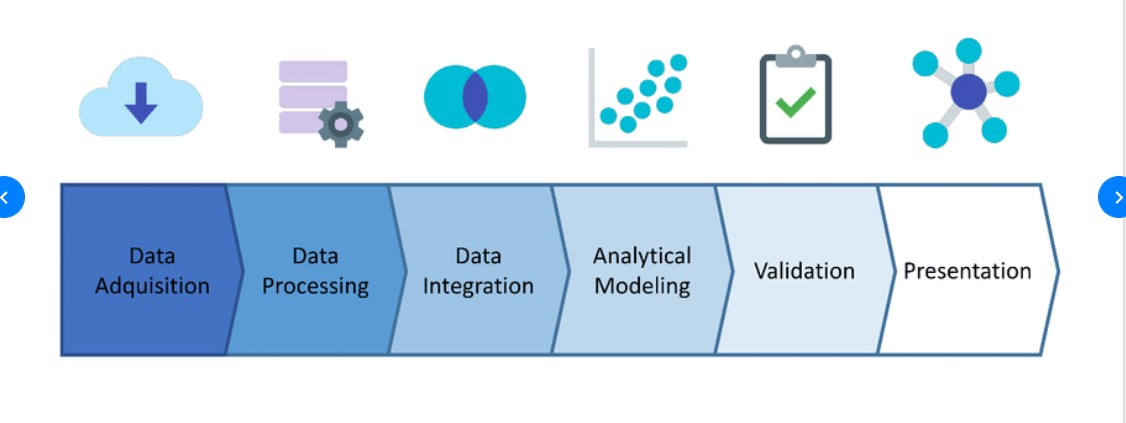
\includegraphics[scale=0.6]{Figs/Fig1.jpg}
\caption[First image phasellus at magna interdum, mattis tellus vitae, varius sapien pellentesque auctor neque ante, sit amet posuere nibh cursus vel]
{First image phasellus at magna interdum, mattis tellus vitae, varius sapien pellentesque auctor neque ante, sit amet posuere nibh cursus vel. Phasellus sed lacinia leo. Only the first sentence of the images and tables should show up in the tables of contents.}
\label{fig:figure1}
\end{figure}

Lorem ipsum dolor sit amet, consectetur adipiscing elit. Ut sed est bibendum, vestibulum enim ac, mattis turpis. Maecenas blandit dui a dui fermentum venenatis. Maecenas posuere augue sed porttitor posuere. Donec vitae tortor faucibus, luctus urna vitae, hendrerit massa. Cras ac dui dui. Etiam euismod vehicula metus, sit amet ultricies massa blandit vitae. Aliquam sodales tempor lorem, ac venenatis diam convallis id. Maecenas ornare vulputate tellus et volutpat. Fusce vehicula nisi ac lorem varius bibendum. Pellentesque viverra ultricies libero, a malesuada augue ultricies nec.

Curabitur vel nisi aliquam, faucibus est sed, semper mi. Praesent eget suscipit lacus. Maecenas fringilla erat vitae tortor imperdiet, eu interdum est molestie. Sed aliquet interdum magna non venenatis. Proin ut elit porta, tincidunt mauris quis, condimentum mauris. Sed in nisi non sem fringilla pharetra. Sed lacinia convallis libero a ultricies. Curabitur varius blandit dui. Cras tempus dignissim elementum. Sed nisl libero, efficitur et nisl nec, fringilla varius libero. Aenean eu dictum nunc, ac convallis turpis. Donec convallis tortor in lectus rhoncus, ac laoreet arcu convallis. Phasellus at magna interdum, mattis tellus vitae, varius sapien. Pellentesque auctor neque ante, sit amet posuere nibh cursus vel. Phasellus sed lacinia leo.
\chapter{CHAPTER 2 TITTLE}
\label{ch:relatedwork}

Lorem ipsum dolor sit amet, consectetur adipiscing elit. Nam in venenatis ligula, eget congue turpis. Praesent ante quam, facilisis at magna sed, lacinia iaculis eros. Aenean id dui augue. Aenean in nibh sollicitudin erat accumsan venenatis id eget magna. Maecenas in metus lorem. Pellentesque id accumsan urna, faucibus volutpat arcu. Fusce tempor lectus quis purus accumsan malesuada.

Citation examples: networkX \cite{SciPyProceedings_11}, scikit-learn \cite{scikit-learn}, and Spectral Clustering tutorial \cite{von2007tutorial}.


\section*{Section 1} 
\addcontentsline{toc}{section}{Section 1}

Curabitur vel nisi aliquam, faucibus est sed, semper mi. Praesent eget suscipit lacus. Maecenas fringilla erat vitae tortor imperdiet, eu interdum est molestie. Sed aliquet interdum magna non venenatis. Proin ut elit porta, tincidunt mauris quis, condimentum mauris. Sed in nisi non sem fringilla pharetra. Sed lacinia convallis libero a ultricies. Curabitur varius blandit dui. Cras tempus dignissim elementum. Sed nisl libero, efficitur et nisl nec, fringilla varius libero. Aenean eu dictum nunc, ac convallis turpis. Donec convallis tortor in lectus rhoncus, ac laoreet arcu convallis. Phasellus at magna interdum, mattis tellus vitae, varius sapien. Pellentesque auctor neque ante, sit amet posuere nibh cursus vel. Phasellus sed lacinia leo. 


\subsection*{Subsection 1} 


Lorem ipsum dolor sit amet, consectetur adipiscing elit. Ut sed est bibendum, vestibulum enim ac, mattis turpis. Maecenas blandit dui a dui fermentum venenatis. Maecenas posuere augue sed porttitor posuere. Donec vitae tortor faucibus, luctus urna vitae, hendrerit massa. Cras ac dui dui. Etiam euismod vehicula metus, sit amet ultricies massa blandit vitae. Aliquam sodales tempor lorem, ac venenatis diam convallis id. Maecenas ornare vulputate tellus et volutpat. Fusce vehicula nisi ac lorem varius bibendum. Pellentesque viverra ultricies libero, a malesuada augue ultricies nec.

Table~\ref{tab:table2} shows...


\begin{table}[ht]
\caption[Second table phasellus at magna interdum, mattis tellus vitae, varius sapien pellentesque auctor neque ante, sit amet posuere nibh cursus vel]
{Second table phasellus at magna interdum, mattis tellus vitae, varius sapien pellentesque auctor neque ante, sit amet posuere nibh cursus vel. Phasellus sed lacinia leo. Only the first sentence of the images and tables should show up in the tables of contents.}
\centering
\fontsize{10}{12}\selectfont
\begin{tabular}{|l|r|r|}
\hline
Dataset name & Number of records  & Number of users \\
\hline 
Dataset A & 248 & 20 \\
\hline
Dataset B & 464 & 28 \\
\hline
Dataset C & 348 & 7 \\
\hline
Dataset D & 419 & 5\\
\hline
Dataset E & 854 & 15\\
\hline
\end{tabular}
\label{tab:table2}
\end{table}


Lorem ipsum dolor sit amet, consectetur adipiscing elit. Ut sed est bibendum, vestibulum enim ac, mattis turpis. Maecenas blandit dui a dui fermentum venenatis. Maecenas posuere augue sed porttitor posuere. Donec vitae tortor faucibus, luctus urna vitae, hendrerit massa. Cras ac dui dui. Etiam euismod vehicula metus, sit amet ultricies massa blandit vitae. Aliquam sodales tempor lorem, ac venenatis diam convallis id. Maecenas ornare vulputate tellus et volutpat. Fusce vehicula nisi ac lorem varius bibendum. Pellentesque viverra ultricies libero, a malesuada augue ultricies nec.

\subsection*{Subsection 2} 

Lorem ipsum dolor sit amet, consectetur adipiscing elit. Ut sed est bibendum, vestibulum enim ac, mattis turpis. Maecenas blandit dui a dui fermentum venenatis. Maecenas posuere augue sed porttitor posuere. Donec vitae tortor faucibus, luctus urna vitae, hendrerit massa. Cras ac dui dui. Etiam euismod vehicula metus, sit amet ultricies massa blandit vitae. Aliquam sodales tempor lorem, ac venenatis diam convallis id. Maecenas ornare vulputate tellus et volutpat. Fusce vehicula nisi ac lorem varius bibendum. Pellentesque viverra ultricies libero, a malesuada augue ultricies nec.



Figure~\ref{fig:figure2} shows...

\begin{figure}[h!]
\centering
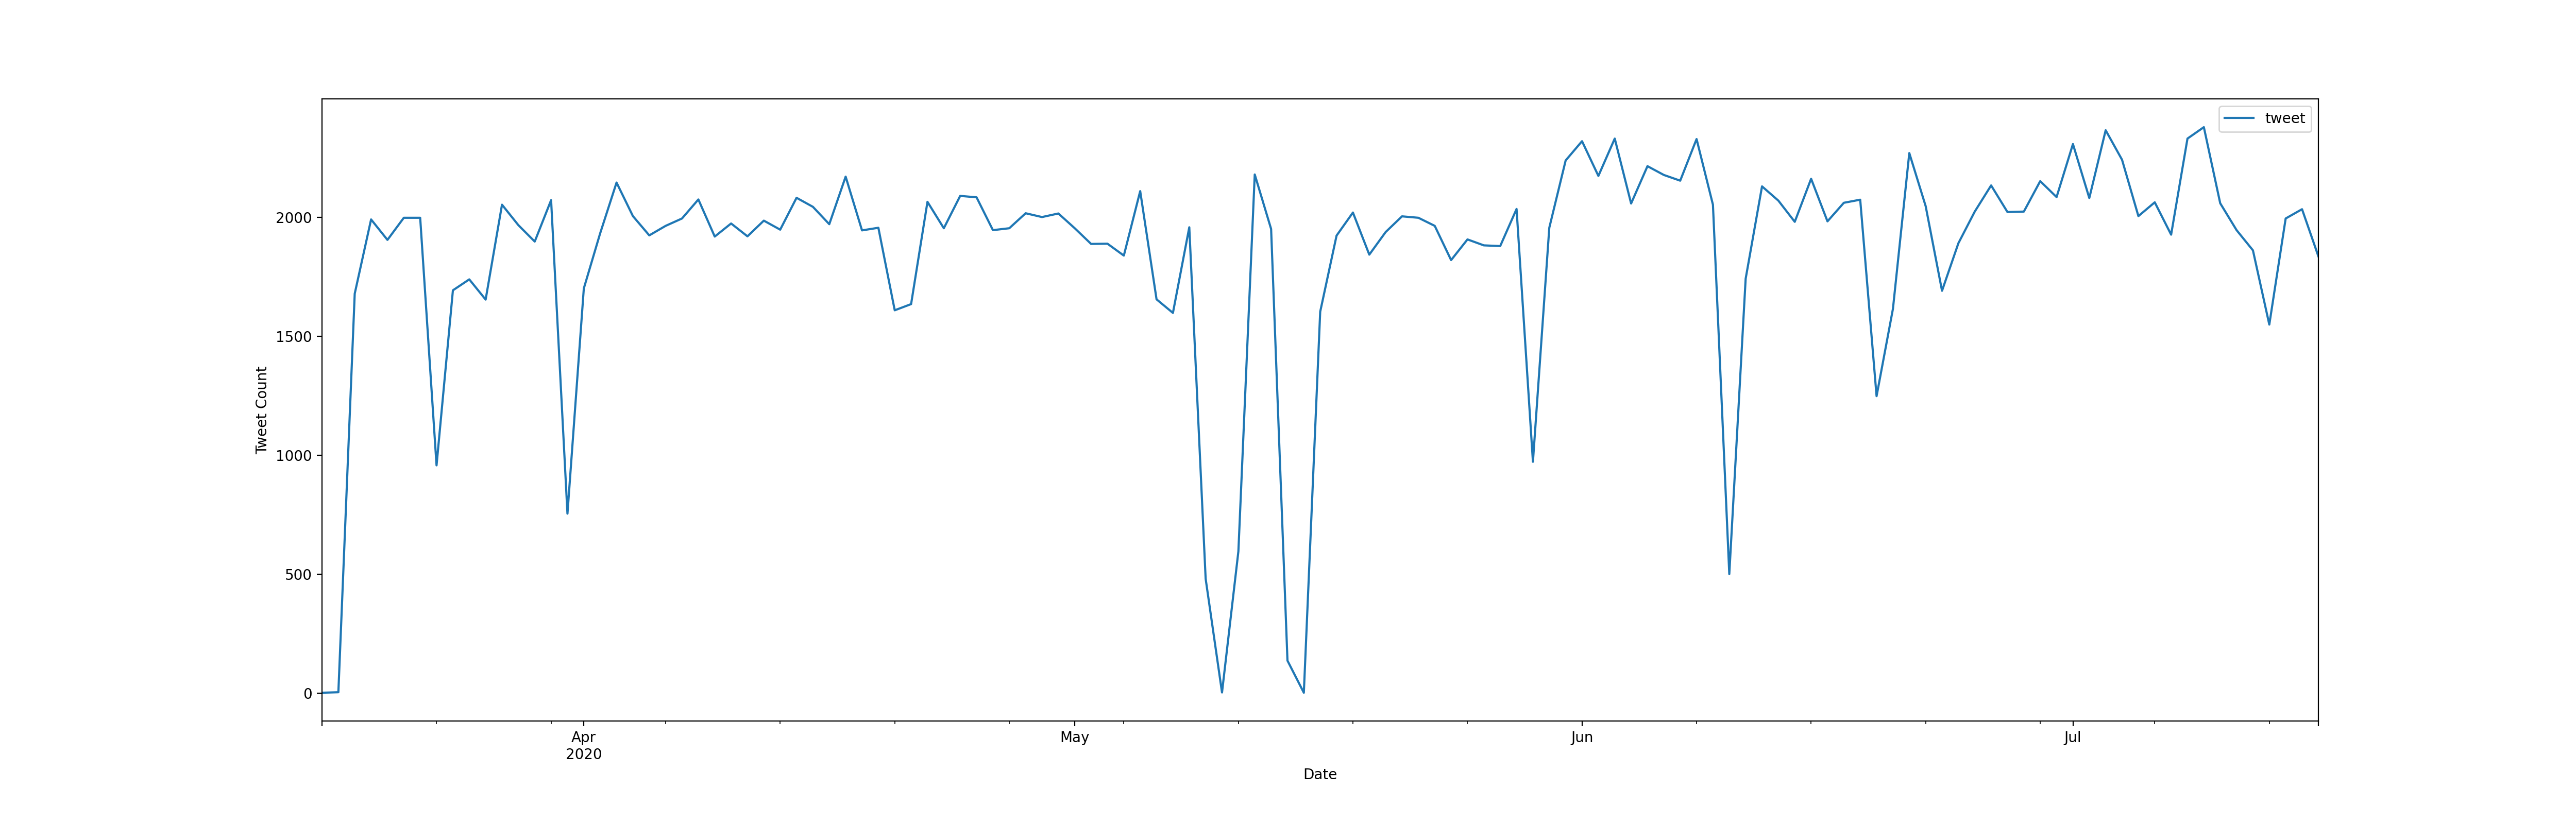
\includegraphics[scale=0.3]{Figs/Fig2.png}
\caption[Second image phasellus at magna interdum, mattis tellus vitae, varius sapien pellentesque auctor neque ante]
{Second image phasellus at magna interdum, mattis tellus vitae, varius sapien pellentesque auctor neque ante. Phasellus sed lacinia leo. Only the first sentence of the images and tables should show up in the tables of contents.}
\label{fig:figure2}
\end{figure}


\section*{Section 2} 
\addcontentsline{toc}{section}{Section 2}

Lorem ipsum dolor sit amet, consectetur adipiscing elit. Ut sed est bibendum, vestibulum enim ac, mattis turpis. Maecenas blandit dui a dui fermentum venenatis. Maecenas posuere augue sed porttitor posuere. Donec vitae tortor faucibus, luctus urna vitae, hendrerit massa. Cras ac dui dui. Etiam euismod vehicula metus, sit amet ultricies massa blandit vitae. Aliquam sodales tempor lorem, ac venenatis diam convallis id. Maecenas ornare vulputate tellus et volutpat. Fusce vehicula nisi ac lorem varius bibendum. Pellentesque viverra ultricies libero, a malesuada augue ultricies nec.





\let\svaddcontentsline\addcontentsline
\renewcommand\addcontentsline[3]{%
  \edef\qtest{#1}%
  \def\qmatch{lof}%
  \ifx\qmatch\qtest\else%
    \def\qmatch{lot}%
    \ifx\qmatch\qtest\else%
      \svaddcontentsline{#1}{#2}{#3}%
  \fi\fi%
}

% Appendix - remove this if you don't have an appendix
\addtocontents{toc}{\cftpagenumberson{part}}
\chapter*{APPENDIX SECTION}
\addcontentsline{toc}{part}{APPENDIX SECTION}
\label{ch:appendix}

% restarts the count of figures and tables
\renewcommand{\thetable}{A.\arabic{table}}  
\renewcommand{\thefigure}{A.\arabic{figure}}
\setcounter{figure}{0}
\setcounter{table}{0}

\begin{center}
APPENDIX A
\end{center}

\begin{figure}[ht]
\centering
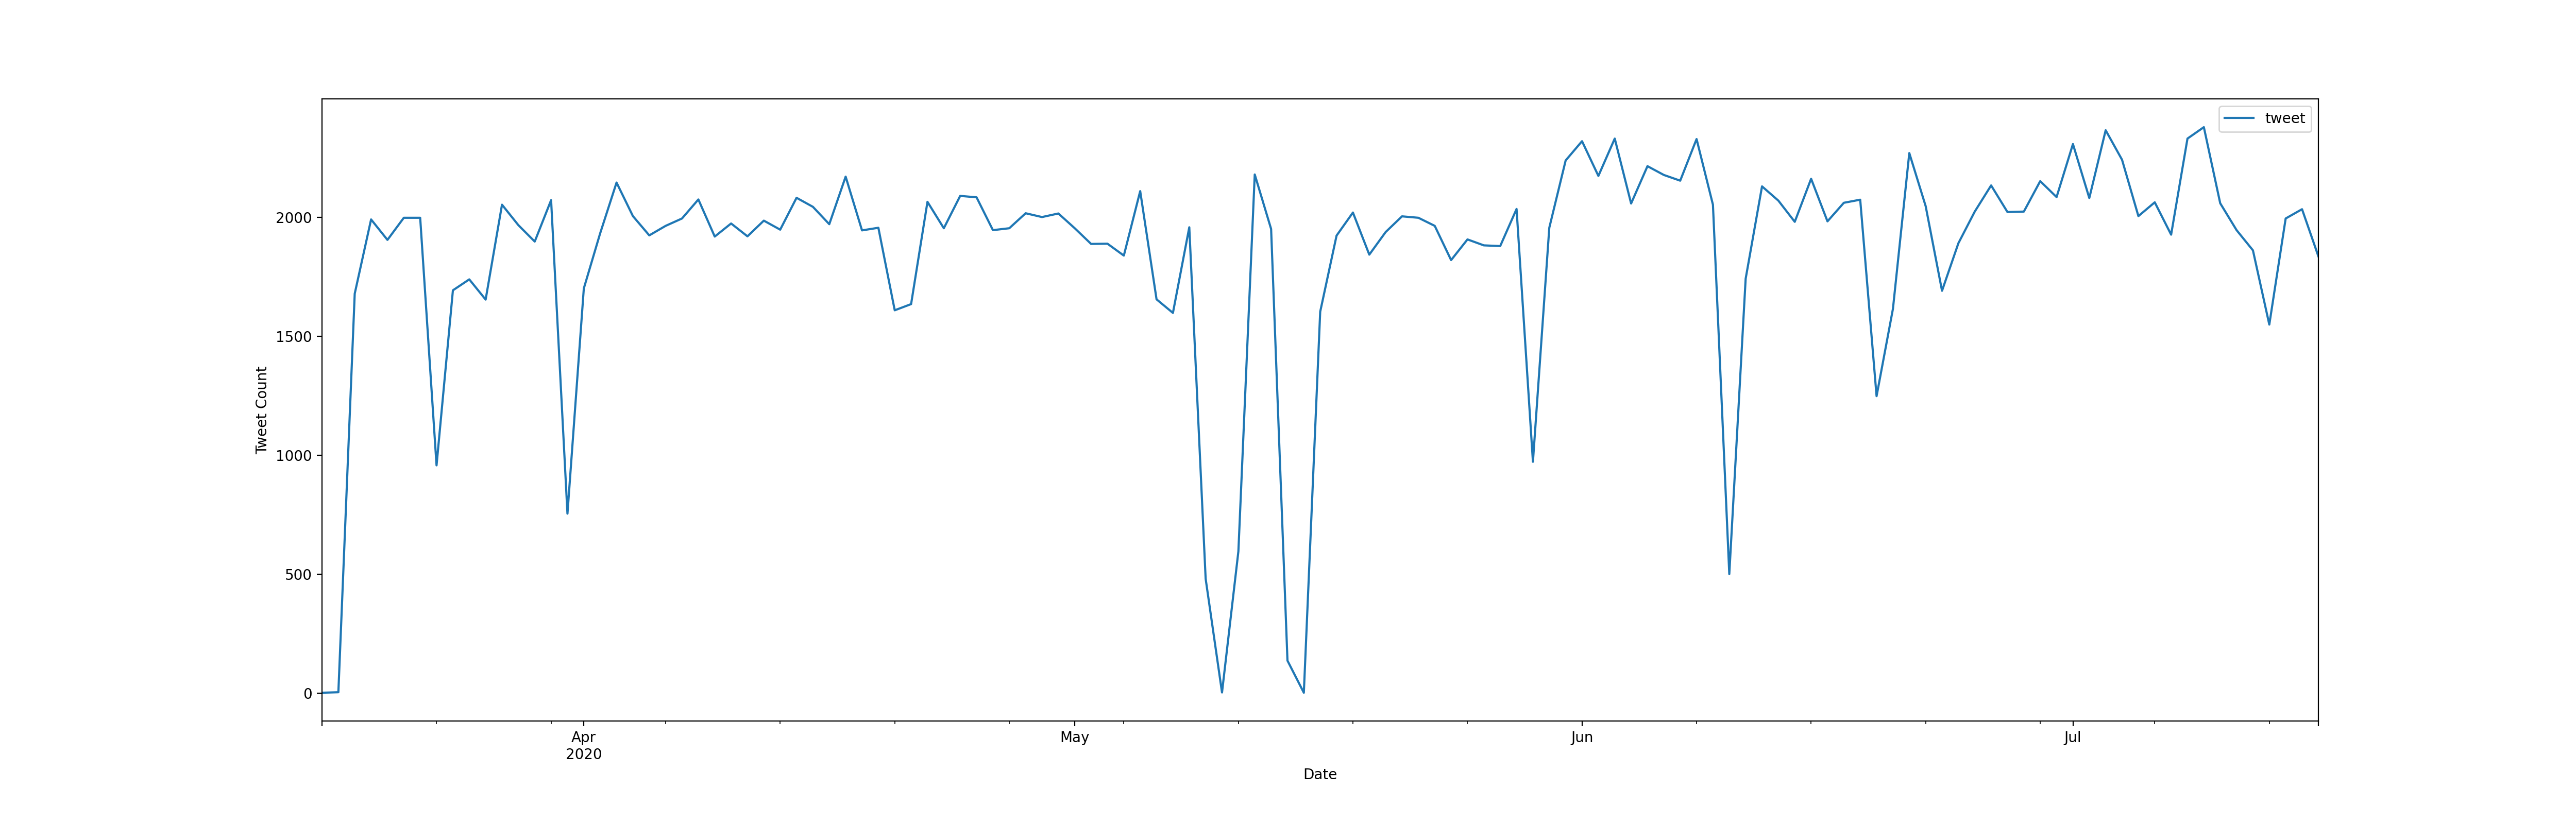
\includegraphics[scale=0.6]{Figs/Fig2.png}
\caption{First figure of appendix A. Captions of figures and tables in the Appendix section should not show up in the table of contents.}
\label{fig:figure1AP}
\end{figure}

\begin{table}[ht]
\caption{First table of appendix A. Captions of figures and tables in the Appendix section should not show up in the table of contents.}
\centering
\fontsize{10}{12}\selectfont
\begin{tabular}{|l|r|r|}
\hline
Dataset name & Number of records  & Number of users \\
\hline 
Dataset A & 248 & 20 \\
\hline
Dataset B & 464 & 28 \\
\hline
Dataset C & 348 & 7 \\
\hline
Dataset D & 419 & 5\\
\hline
Dataset E & 854 & 15\\
\hline
\end{tabular}
\label{tab:table1AP}
\end{table}


\begin{table}[ht]
\caption{Second table of appendix A. Captions of figures and tables in the Appendix section should not show up in the table of contents.}
\centering
\fontsize{10}{12}\selectfont
\begin{tabular}{|l|r|r|}
\hline
Dataset name & Number of records  & Number of users \\
\hline 
Dataset F & 1000 & 10 \\
\hline
Dataset G & 2000 & 20 \\
\hline
Dataset H & 3000 & 30 \\
\hline
Dataset I & 4000 & 40\\
\hline
Dataset J & 5000 & 50\\
\hline
\end{tabular}
\label{tab:table2AP}
\end{table}



\clearpage
\pagebreak


% restarts the count of figures and tables
\renewcommand{\thetable}{B.\arabic{table}}  
\renewcommand{\thefigure}{B.\arabic{figure}}
\setcounter{figure}{0}
\setcounter{table}{0}


\FloatBarrier
\begin{center}
APPENDIX B
\end{center}


\begin{table}[ht]
\caption{First table of appendix B. Captions of figures and tables in the Appendix section should not show up in the table of contents.}
\centering
\fontsize{10}{12}\selectfont
\begin{tabular}{|l|r|r|}
\hline
Column 1 & Column 2  & Column 3 \\
\hline 
1 & 2 & 10000 \\
\hline
3 & 4 & 20000 \\
\hline
5 & 6 & 30000 \\
\hline
\end{tabular}
\label{tab:table3AP}
\end{table}


\begin{table}[ht]
\caption{Second figure of appendix B. Captions of figures and tables in the Appendix section should not show up in the table of contents.}
\centering
\fontsize{10}{12}\selectfont
\begin{tabular}{|l|r|r|}
\hline
Column 1 & Column 2  & Column 3 \\
\hline 
A & B & 10000 \\
\hline
C & D & 20000 \\
\hline
E & F & 30000 \\
\hline
\end{tabular}
\label{tab:table4AP}
\end{table}


\begin{figure}[ht]
\centering
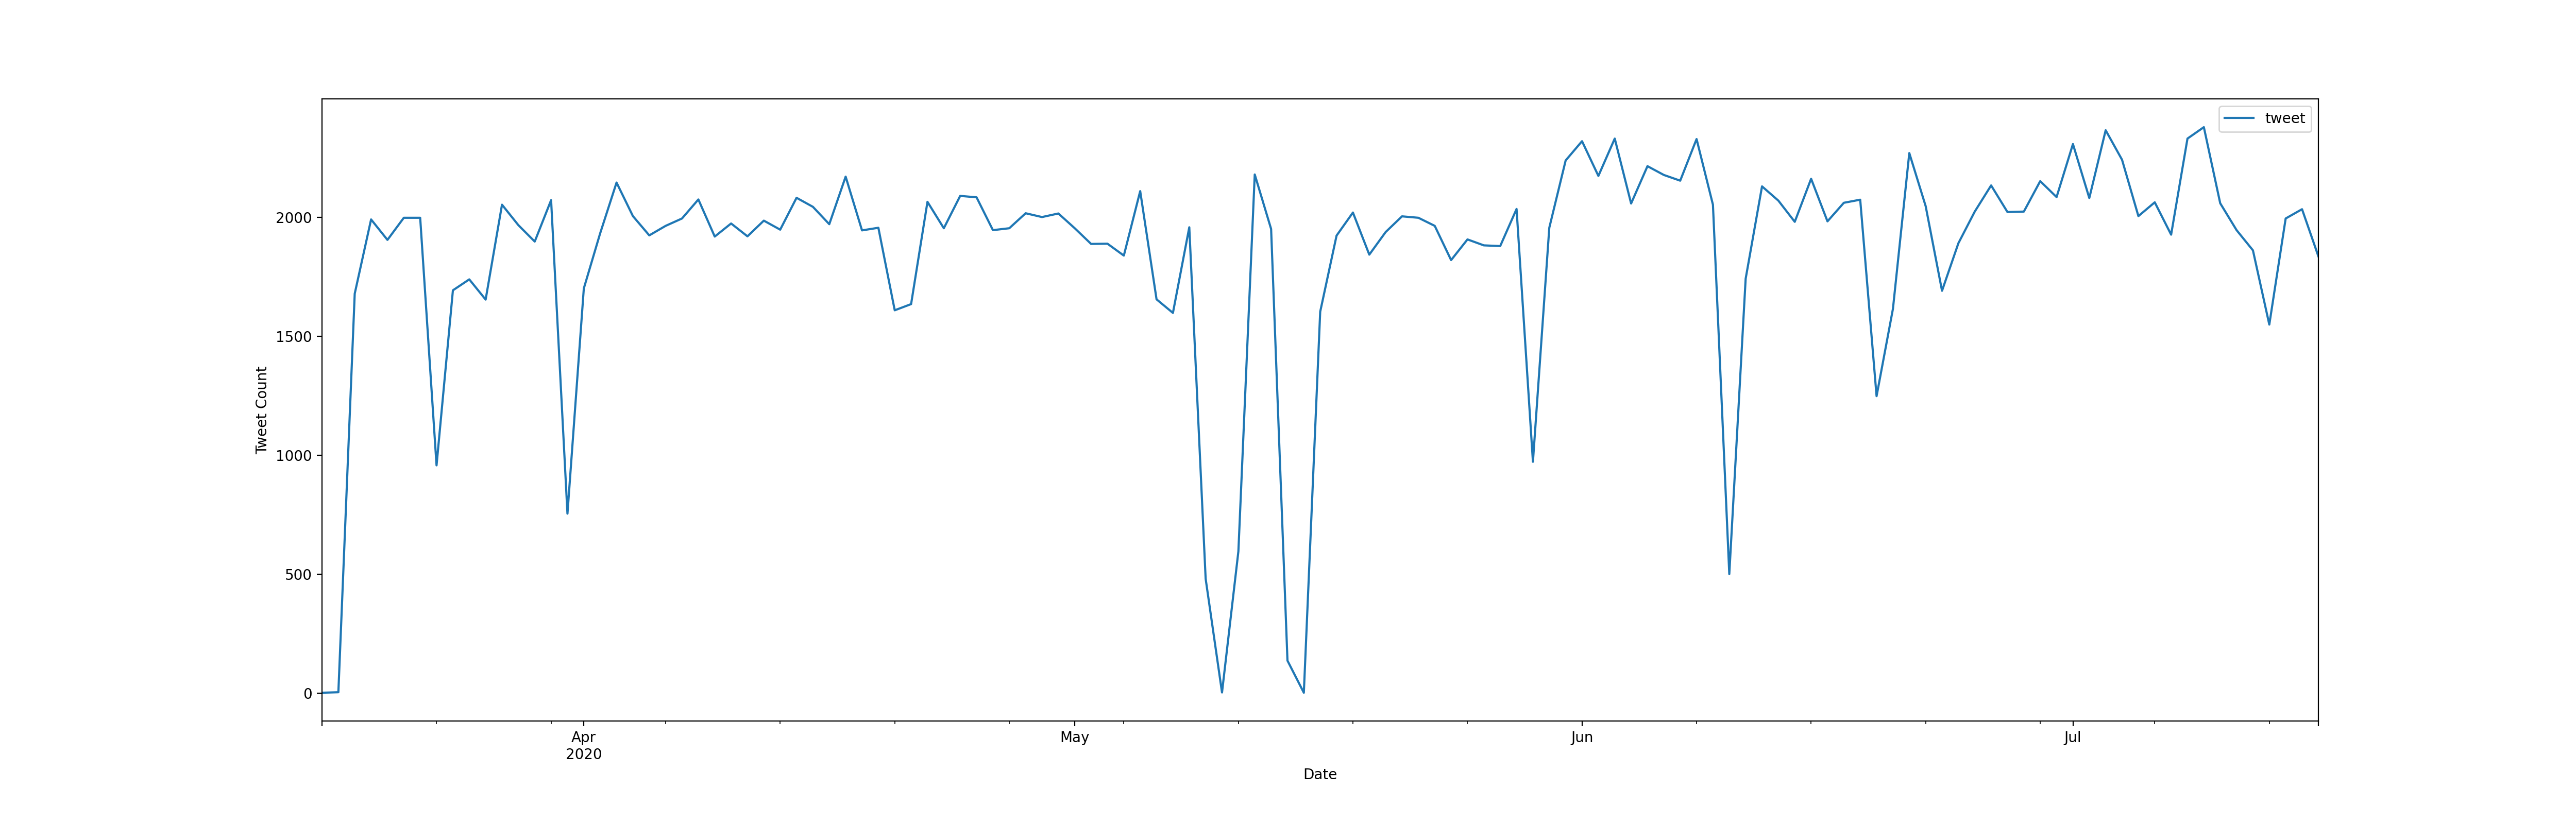
\includegraphics[scale=0.22]{Figs/Fig2.png}
\caption{First figure of appendix B. Captions of figures and tables in the Appendix section should not show up in the table of contents.}
\label{fig:figure3AP}
\end{figure}






%********************************************************************
% Other Stuff in the Back
%*******************************************************
\singlespacing
%********************************************************************
% Bibliography
%*******************************************************
\phantomsection 
\refstepcounter{dummy}
\addcontentsline{toc}{part}{REFERENCES}
\bibliographystyle{ieeetr}
\bibliography{./Bib/References}


% ********************************************************************
% Game Over: Restore, Restart, or Quit?
%*******************************************************
\end{document}
% ********************************************************************
